\chapter{基于声场扩阶的双耳渲染算法 }\label{chapter.AddWindow}

由于实际情况的限制,基于球谐分解的双耳渲染算法在声场和~HRTF~之间存在不匹配问题,第~\ref{chapter.HRTF}~章中对~HRTF~进行相位对准预处理,以降低~HRTF~的球谐分解阶次。声场在算法中和~HRTF~有着同等重要的地位, 但是目前的算法均集中于~HRTF~预处理。本章将从声场角度出发,提出一种新的声场扩阶算法,以提升声场的球谐分解阶次。首先对信号模型进行介绍,其次对声场扩阶算法的原理进行详细介绍,即通过对原始录制声场进行空域加窗,以实现对录制声场分解阶次的提升,接下来对本文采用的空域窗函数加以介绍。并且将声场扩阶方法与~HRTF~预处理方法相结合,给出整体算法框图,共同解决目前双耳渲染中存在的问题。

\section{信号模型}\label{sec.modelAndMusic}
% 可以加入: 即使同时存在两个语音信息,在大多数时频点也只有一个声源。参见test或者球阵定位的相关文章。

考虑位于远场的一个声源信号和~$Q$~个麦克风,将麦克风在某个时频点上的接收信号建模为:
\begin{equation}\label{eq.model}
\bm{S} = \bm{S}_{p} + \bm{S}_{d},
\end{equation}
其中,第一项~$\bm{S}_{p}$~表示平面波,与声源的方位相关。其中,声源方位可以是直达波,也可以是早期反射,描述为在该时频点上能量较大的信号。第二项~$\bm{S}_{d}$~表示扩散声场(diffuse filed),由来自许多方向的不相关的平面波组成。第一项和第二项分别表示声源分量和环境分量。

该模型假设来源于语音信号的稀疏性。对于语音信号来说,常采用短时傅里叶变换(Short Time Fourier Transform,STFT),其在时频域上具有稀疏性,语音能量不仅集中在少数时间帧上,更集中在少量的时频单元上。

其中,第一项~$\bm{S}_{p}$~对应的声源方位可以通过许多方法进行获取,估计声源的到达方向(direction of arrival,DOA)一直是人们关注的领域。基于波束形成、最大似然以及子空间方法等各种~DOA~估计方法之前已被广泛研究,并且在球形麦克风阵列上加以扩展~\tcite{2012Localization},接下来将简单介绍。

MUSIC~方法是非常经典的子空间~DOA~方法,其算法简单、高空间分辨率高,是目前比较流行的~DOA~估计算法之一,基于球形麦克风阵列的~MUSIC~方法可以在空域和球谐域上进行,本文主要关注基于球阵的球谐域~MUSIC~算法。对球形麦克风阵列的采集信号进行~SH~变换转换到球谐域的好处是,与传统的空域~MUSIC~算法相比,球谐域~MUSIC~算法通过解耦去除球谐域中与频率相关的分量,其阵列流形矩阵与频率无关,独立于阵列设置,且计算简单~\tcite{2012Localization}。

假设有~$J$~个幅度为~$s_{j}(f)$,来波方向为~$(\theta_{j},\phi_{j})$~的平面波,由公式~\eqref{SMic_pressure}~可得,第~$q$~个麦克风的接收信号和其球谐分解系数分别为:
\begin{equation}
   S(r,\theta_q,\phi_q,f)=
   \sum _{n=0}^{\infty}\sum _{m=-n}^{n}\sum_{j=1}^{J} s_{j}(f) b_n(kr) Y_n ^{m}(\theta_q,\phi_q) [Y_n ^{m}(\theta_j,\phi_j)]^{*},
\end{equation}
和
\begin{equation}\label{eq.Snm_Jplane}
   S_n ^m(r,f) =
    b_n(kr) \sum_{j=1}^{J} s_{j}(f) [Y_n ^{m}(\theta_j,\phi_j)]^{*}.
\end{equation}

定义~$s_n ^m(f) = S_n ^m(r,f) / b_n(kr)$~,式~\eqref{eq.Snm_Jplane}~可写为:
\begin{equation}
   s_n^m(f) =
    \sum_{j=1}^{J} s_{j}(f) [Y_n ^{m}(\theta_j,\phi_j)]^{*},
\end{equation}
其矩阵形式为:
\begin{equation}
   \bm{s_n^m} =
    \bm{Y^{H} s},
\end{equation}
其中,$\bm{s_n^m}$~是一个长度为~$(N_{s}+1)^2$~的向量:
\begin{equation}
\bm{s_n^m} = [~s_{0}^{0}(f)~,~s_{1}^{-1}(f)~,~s_{1}^{0}(f)~,~s_{1}^{1}(f)~,~\cdots~,~~s_{N_{s}}^{N_{s}}(f)]^{T},
\end{equation}
$\bm{s}$~是一个长度为~$J$~的平面波幅度向量:
\begin{equation}
\bm{s} = [~s_{1}(f)~,~s_{2}(f)~,~\cdots~,~s_{J}(f)~]^{T},
\end{equation}
$\bm{Y}$~是一个~$J\times(N_{s}+1)^2$~的球谐域流形矩阵,其中第~$j$~行为声源位于~$(\theta_{j},\phi_{j})$~方位处的球谐域流行向量,表示为:
\begin{equation}\label{eq.y}
\mathbf{y}(\theta_{j},\phi_{j}) = [~Y_{0}^{0}(\theta_{j},\phi_{j})~,~\cdots~,~Y_{n}^{m}(\theta_{j},\phi_{j})~,~Y_{N_{s}}^{N_{s}}(\theta_{j},\phi_{j})~]
\end{equation}
由式~\eqref{eq.y}~可知,球谐域~MUSIC~算法的阵列流形矩阵与频率无关,且独立于阵列设置,即与麦克风所在位置无关。

相关谱矩阵可以由下式得到:
\begin{equation}
\hat{\mathbf{S}}=\bm{s_n^m} [\bm{s_n^m}]^{H}
\end{equation}
则~MUSIC~谱函数可以表示为:
\begin{equation}
P_{MU}(\theta,\phi)=\frac{1}{\mathbf{y}(\theta,\phi) \mathbf{E}_{N_{s}} \mathbf{E}_{N_{s}}^{H} \mathbf{y}^{H}(\theta,\phi)},
\end{equation}
其中,矩阵~$\mathbf{E}_{N_{s}}$~是噪声子空间,每一列对应一个噪声特征向量,是矩阵~$\hat{\mathbf{S}}$~最小的~$(N_{s}+1)^2-J $~个特征值对应的特征向量,这些特征向量可以通过对矩阵~$\hat{\mathbf{S}}$~进行特征值分解获得。令~$(\theta,\phi)$~在空间中变化,搜索~$P_{MU}(\theta,\phi)$~的~$J$~个峰值,对应的角度即为平面波来波方向的估计值。

在本文中,如式~\eqref{eq.model}~所示,假设每一个时频点只存在一个平面波,此时~$J=1$,噪声子空间中特征向量的数目为~$(N_{s}+1)^2-1 $。

在此对球贝塞尔函数的零点问题(如图~\ref{fig:bn}~所示)给定位算法带来的影响加以讨论。如上述定义~$s_n ^m(f) = S_n ^m(r,f) / b_n(kr)$~所示,使用球谐域~MUSIC~算法进行定位时需要对所获取的球谐分量~$S_n ^m(r,f)$~除以~$b_{n}(kr)$。对于单个空心球来说,即需要除以~$j_{n}(kr)$,这将导致~$s_n ^m(f)$~为一极大值,带来很大的定位误差。对于刚性球来说,则可以很好地避免这个问题。


\section{声场扩阶原理}

本节将对所提出的声场扩阶原理进行详细介绍,首先给出了有界线性算子及其在球谐域的表示形式,以此为基础对空域加窗算子在球谐域上的表示进行了详细推导,得到加窗后信号的球谐系数表达式,并且对空域加窗带来的声场扩阶现象加以分析。

\subsection{有界线性算子}
对于一个在~$L^{2}(\mathbb{S}^{2})$~空间的有界线性算子~$\mathcal{B}$~\tcite{Hilbert},将~$S(\theta,\phi)$~映射到~$G(\theta,\phi)$(简便起见,麦克风位置~$r$~和频率~$f$~省略不写),记作:
\begin{equation}
G(\theta,\phi) = \left(\mathcal{B} S\right) (\theta,\phi)
\end{equation}
也可以简记为~$G = \mathcal{B} S $。在大多数情况下,$\mathcal{B}$~用于表示一个通用的有界操作符,或者在特定有界运算符的表示中用作统称。

在可分离的希尔伯特空间,对于一个给定的完备正交序列~$\{\psi\}_{n=1}^{\infty}$,任意一个有界线性算子~$\mathcal{B}$~可以使用一个无限矩阵~$\mathbf{B}^{(\psi)}$~等价表示。矩阵在第~$n$~行~$m$~列的元素~$b_{n,m}^{(\psi)}$~表示沿着~$\psi_{m}$~方向的输入与经过该有界线性算子~$\mathcal{B}$~后沿着~$\psi_{n}$~方向的输出之间的关系。

由于~$L^{2}(\mathbb{S}^{2})$~空间是可分离的,并且球谐函数是一个完备正交序列。因此,可以结合球谐分解得到有界线性算子在球谐域的表示形式。映射前后的信号可表示为:
\begin{equation}\label{S_pq_infty}
S(\theta,\phi) = \sum_{n=0}^{\infty}\sum_{m=-n}^{n} S_{n}^{m} Y_{n}^{m}(\theta,\phi).
\end{equation}
\begin{equation}\label{G_lm_infty}
G(\theta,\phi) =  \sum_{p=0}^{\infty} \sum_{q=-p}^{p} G_{p}^{q} Y_{p}^{q}(\theta,\phi).
\end{equation}

我们几乎只用球谐函数作为完备正交序列,因此可以去掉对基函数上标~$\psi$~的依赖性,简单地把~$\mathbf{B}^{(\psi)}$~写成~$\mathbf{B}$~的形式。

此时,算子~$\mathcal{B}$~可以用无限矩阵~$\mathbf{B}$~表示,其矩阵元素~$b_{p,n}^{q,m}$~表示的是以~$Y_{n}^{m}$~为输入,
经过算子~$\mathcal{B}$~后输出信号在~$Y_{p}^{q}$~方向的分量,表示为:
\begin{equation}\label{eq.b_lmpq}
b_{p,n}^{q,m} = \left< \mathcal{B}Y_{n}^{m},Y_{p}^{q} \right>,
\end{equation}
其中,$\left< \cdot \right>$~表示内积,式~\eqref{eq.b_lmpq}~可进一步表示为:

\begin{equation}
b_{p,n}^{q,m} = \int_{0}^{2\pi}\int _{0}^{\pi} B(\theta,\phi)Y_{n}^{m}(\theta,\phi) \left[Y_{p}^{q}(\theta,\phi) \right]^{*}\sin\theta d\theta d\phi
\end{equation}

在式~\eqref{eq.b_lmpq}~中,一对~$m$~和~$n$~对应矩阵~$\mathbf{B}$~的一列,即第~$n^2+n+m+1$~列,一对~$p$~和~$q$~对应矩阵~$\mathbf{B}$~的一行,即第~$p^2+p+q+1$~行,算子矩阵~$\mathbf{B}$~如下所示:

\begin{align}
\mathbf{B} & =\left[
\begin{array}{cccc}
b_{0,0} & b_{0,1} & b_{0,2} & \cdots  \\
b_{1,0} & b_{1,1} & b_{1,2} & \cdots  \\
b_{2,0} & b_{2,1} & b_{2,2} & \cdots   \\
\vdots & \vdots &  \vdots  & \ddots
\end{array}\right]
= \left[
\begin{array}{c|ccc|cc}
b_{0,0}^{0,0} & b_{0,1}^{0,-1} & b_{0,1}^{0,0} & b_{0,1}^{0,1} & b_{0,2}^{0,-2} & \cdots  \\
\hline
b_{1,0}^{-1,0} & b_{1,1}^{-1,-1} & b_{1,1}^{-1,0} & b_{1,1}^{-1,1} & b_{1,2}^{-1,-2} & \cdots  \\
b_{1,0}^{0,0} & b_{1,1}^{0,-1} & b_{1,1}^{0,0} & b_{1,1}^{0,1} & b_{1,2}^{0,-2} & \cdots  \\
b_{1,0}^{1,0} & b_{1,1}^{1,-1} & b_{1,1}^{1,0} & b_{1,1}^{1,1} & b_{1,2}^{1,-2} & \cdots  \\
\hline
b_{2,0}^{-2,0} & b_{2,1}^{-2,-1} & b_{2,1}^{-2,0} & b_{2,1}^{-2,1} & b_{2,2}^{-2,-2} & \cdots  \\
\vdots & \vdots &  \vdots  & \vdots &  \vdots & \ddots
\end{array}\right].
\end{align}

因此有界算子~$\mathcal{B}$~将~$S\in L^{2}\left(\mathbb{S}^{2}\right)$~的球谐系数~$S_ {n}^{m}=\left< S, Y_{n}^{m}\right> $~映射到~$G \in L^{2}\left(\mathbb{S}^{2}\right)$~的球谐系数~$G_{p}^{q} = \left<G,Y_{p}^{q}\right> = \left<\mathcal{B}S,Y_{p}^{q}\right>$,则~$G_{p}^{q} $~和~$G(\theta,\phi)$~可以表示为:
\begin{equation}\label{eq.G_lm}
G_{p}^{q}  = \sum_{n=0}^{\infty}\sum_{m=-n}^{n} S_{n}^{m} b_{p,n}^{q,m}
\end{equation}
\begin{equation}
G(\theta,\phi) = \sum_{p=0}^{\infty} \sum_{q=-p}^{p}\sum_{n=0}^{\infty}\sum_{m=-n}^{n} S_{n}^{m} b_{p,n}^{q,m} Y_{p}^{q}(\theta,\phi)
\end{equation}

对于复合算子~$\mathcal{P = B \cdot D }$,其算子矩阵可以简单地由各个算子的算子矩阵给出,其算子矩阵元素可表示为:
\begin{equation}
p_{p,s}^{q,t} = \sum_{n=0}^{\infty} \sum_{m=-n}^{m} b_{p,n}^{q,m} d_{n,s}^{m,t},
\end{equation}
其中,$p_{p,s}^{q,t}$、$b_{p,n}^{q,m}$~和~$d_{n,s}^{m,t}$~分别为~$\mathcal{P}$、$\mathcal{B}$~和~$\mathcal{D}$~的算子矩阵元素。

\subsection{空域加窗}\label{subsec.Addwindow}
在空间域使用窗函数对一个信号进行掩蔽,即将感兴趣的信号~$S(\theta,\phi)$~与设计合理的窗函数~$h(\theta,\phi)$~在空间域上逐点相乘。将空域加窗对应的空间掩蔽算子记为~$\mathcal{B}_{h}$~,则加窗后信号在空间域的表达式为:
\begin{equation}
\left( \mathcal{B}_{h} S\right)(\theta,\phi) = h(\theta,\phi)S(\theta,\phi),
\end{equation}
其中,$h(\theta,\phi)$~为空域窗函数。

空间掩蔽算子~$\mathcal{B}_{h}$~对应的算子矩阵元素为:
\begin{equation}
b_{p,n}^{q,m} = \int_{0}^{2\pi}\int _{0}^{\pi} h(\theta,\phi)Y_{n}^{m}(\theta,\phi) \left[Y_{p}^{q}(\theta,\phi) \right]^{*}\sin\theta d\theta d\phi.
\end{equation}


与式~\eqref{S_pq_infty}~和~\eqref{G_lm_infty}~类似,对窗函数~$h(\theta,\phi)$~进行球谐分解:
\begin{equation}\label{h_st_infty}
h(\theta,\phi) = \sum_{s=0}^{\infty} \sum_{t=-s}^{s} h_{s}^{t} Y_{s}^{t}(\theta,\phi)
\end{equation}
其中,$h_{s}^{t}$~为窗函数的球谐系数。

因此式~\eqref{eq.G_lm}~可以表示为:
\begin{align}
G_{p}^{q} &= \sum_{n=0}^{\infty}\sum_{m=-n}^{n} S_{n}^{m} b_{p,n}^{q,m} \nonumber \\
& = \sum_{n=0}^{\infty}\sum_{m=-n}^{n}  S_{n}^{m}\int_{0}^{2\pi}\int _{0}^{\pi} h(\theta,\phi)Y_{n}^{m}(\theta,\phi) \left[Y_{p}^{q}(\theta,\phi) \right]^{*}\sin\theta d\theta d\phi \nonumber \\
& = \sum_{n=0}^{\infty}\sum_{m=-n}^{n}  S_{n}^{m}\int_{0}^{2\pi}\int _{0}^{\pi} \sum_{s=0}^{\infty} \sum_{t=-s}^{s} h_{s}^{t} Y_{s}^{t}(\theta,\phi) Y_{n}^{m}(\theta,\phi) \left[Y_{p}^{q}(\theta,\phi) \right]^{*}\sin\theta d\theta d\phi \nonumber \\
& = \sum_{n=0}^{\infty}\sum_{m=-n}^{n} S_{n}^{m}\sum_{s=0}^{\infty} \sum_{t=-s}^{s} h_{s}^{t}\int_{0}^{2\pi}\int _{0}^{\pi}Y_{s}^{t}(\theta,\phi) Y_{n}^{m}(\theta,\phi) \left[Y_{p}^{q}(\theta,\phi) \right]^{*}\sin\theta d\theta d\phi
\end{align}

为上式的积分定义一个简记法:
\begin{equation}\label{y_stlmpq}
y(s,t;n,m;p,q) \triangleq \int_{0}^{2\pi}\int _{0}^{\pi}Y_{s}^{t}(\theta,\phi) Y_{n}^{m}(\theta,\phi) \left[Y_{p}^{q}(\theta,\phi) \right]^{*}\sin\theta d\theta d\phi,
\end{equation}
此时,空间掩蔽算子~$\mathcal{B}_{h}$~对应的算子矩阵元素为:
\begin{equation}
b_{p,n}^{q,m} = \sum_{s=0}^{\infty} \sum_{t=-s}^{s} h_{s}^{t} y(s,t;n,m;p,q).
\end{equation}
加窗后信号的球谐分解系数可以简洁表示为:
\begin{equation}\label{eq.AddWindow_infty}
G_{p}^{q} = \sum_{n=0}^{\infty} \sum_{m=-n}^{n} S_{n}^{m}\sum_{s=0}^{\infty} \sum_{t=-s}^{s} h_{s}^{t}y(s,t;n,m;p,q).
\end{equation}

在量子力学中经常出现包含三个球谐函数的积分,可以用~Wigner~$3j$~符号表示~\tcite{Wigner_3j},式~\eqref{y_stlmpq}~可表示为:
\begin{equation}
y(s,t;n,m;p,q) = (-1)^{q} \sqrt{\frac{(2 s+1)(2 n+1)(2 p+1)}{4 \pi}}\left(\begin{array}{ccc}
s & n & p \\
0 & 0 & 0
\end{array}\right)\left(\begin{array}{ccc}
s & n & p \\
t & m & -q
\end{array}\right),
\end{equation}
其中,后两项不是矩阵,而是~Wigner~$3j$~符号,将在下文对该符号的定义和计算公式进行简单介绍。


Wigner~$3j$~符号是~Wigner~在文献~\cite{Wigner_3j}~中定义的~$3j$~符号,定义为:
\begin{equation}
\left(\begin{array}{ccc}
j_{1} & j_{2} & j_{3} \\
m_{1} & m_{2} & m_{3}
\end{array}\right) \triangleq \frac{(-1)^{j_{1}-j_{2}-m_{3}}}{\sqrt{2 j_{3}+1}} s_{j_{3}, m_{1}, m_{2}}^{j_{1}, j_{2}} \delta_{m_{1}+m_{2}+m_{3}, 0} ,
\end{equation}
其中~$s_{j 3, m_{1}, m_{2}}^{j_{1}, j_{2}}$~的表达式为:
\begin{align*}
s_{j_{3}, m_{1}, m_{2}}^{j_{1}, j_{2}} &=
\frac{\sqrt{\left(j_{3}+j_{1}-j_{2}\right) !\left(j_{3}-j_{1}+j_{2}\right) !\left(j_{1}+j_{2}-j_{3}\right) !\left(j_{3}-m_{3}\right) !\left(j_{3}+m_{3}\right) !}}{\sqrt{\left(j_{1}+j_{2}+j_{3}+1\right) !\left(j_{1}-m_{1}\right) !\left(j_{1}+m_{1}\right) !\left(j_{2}-m_{2}\right) !\left(j_{2}+m_{2}\right) !}}
\end{align*}
\begin{align*}
&  \times \sum_{t} \frac{(-1)^{t+j_{2}+m_{2}} \sqrt{2 j_{3}+1}\left(j_{3}+j_{2}+m_{1}-t\right) !\left(j_{1}-m_{1}+t\right) !}{\left(j_{3}-j_{1}+j_{2}-t\right) !\left(j_{3}-m_{3}-t\right) !(t) !\left(j_{1}-j_{2}+m_{3}+t\right) !}
\end{align*}
在关于~$t$~的求和项中要求所有阶乘内的参数都是非负的。

必须同时满足以下条件,Wigner~$3j$~符号才不是非零值:
\begin{equation}\label{eigner_if}
\begin{split}
m_{1}+m_{2}+m_{3}  = 0 \\
|j_{2}-j_{3}|  \leq j_{1}  \leq j_{2}+j_{3} \\
|j_{1}-j_{3}|  \leq j_{2}  \leq j_{1}+j_{3} \\
|j_{1}-j_{2}|  \leq j_{3}  \leq j_{1}+j_{2} \\
|m_{k}| \leq j_{k}~~,k = 1,2,3
\end{split}
\end{equation}

定义和计算Wigner~$3j$~符号的方法还有很多,其中最广泛使用的是~Racah~公式~\tcite{messiah1961quantum}:
\begin{equation}
\begin{array}{l}
\left(\begin{array}{ccc}
j_{1} & j_{2} & j_{3} \\
m_{1} & m_{2} & m_{3}
\end{array}\right)
=(-1)^{j_{1}-j_{2}-m_{3}} \sqrt{\Delta\left(j_{1}, j_{2}, j_{3}\right)} \\
\times \sqrt{\left(j_{1}-m_{1}\right) !\left(j_{1}+m_{1}\right) !\left(j_{2}-m_{2}\right) !\left(j_{2}+m_{2}\right) !\left(j_{3}-m_{3}\right) !\left(j_{3}+m_{3}\right) !} \\
\end{array}
\end{equation}
\begin{equation*}
\times \sum_{t} \frac{(-1)^{t}}{(t) !\left(j_{1}+j_{2}-j_{3}-t\right) !\left(j_{1}-m_{1}-t\right) !\left(j_{2}+m_{2}-t\right) !\left(j_{3}-j_{2}+m_{1}+t\right) !\left(j_{3}-j_{1}-m_{2}+t\right) !}
\end{equation*}
\\
其中~$\Delta\left(j_{1}, j_{2}, j_{3}\right)$~的表达式为:
\begin{equation*}
\Delta\left(j_{1}, j_{2}, j_{3}\right)=\frac{\left(j_{1}+j_{2}-j_{3}\right) !\left(j_{1}-j_{2}+j_{3}\right) !\left(j_{2}-j_{1}+j_{3}\right) !}{\left(j_{1}+j_{2}+j_{3}+1\right) !}
\end{equation*}

\subsection{空域加窗后的声场阶次}\label{sec.Enlarge_order}

在实际情况中,需要对式~\eqref{S_pq_infty}\eqref{G_lm_infty}\eqref{h_st_infty}~进行截断处理,假设加窗前信号、加窗后信号和窗函数球谐分解的最高阶次分别为~$N_{s}$、$N_{g}$~和~$N_{h'}$,由式~\eqref{eq.AddWindow_N}~可知~$N_{g}$~是由~$N_{s}$~和~$N_{h'}$~共同决定的。
\begin{equation}\label{eq.AddWindow_N}
G_{p}^{q} = \sum_{n=0}^{N_{s}} \sum_{m=-n}^{n} S_{n}^{m}\sum_{s=0}^{N_{h'}} \sum_{t=-s}^{s} h_{s}^{t}y(s,t;n,m;p,q)~,~~~~ 0\leq p \leq N_{g}.
\end{equation}

对于轴对称问题,即窗函数沿水平角~$\phi$~为常数的特殊情况,$N_{s}$、$N_{g}$~和~$N_{h'}$~有显示关系式。此时~$h(\theta,\phi) =h(\theta)$,窗函数的球谐系数为:

\begin{align}\label{h_st_constant}
h_{s}^{t} & = \int_{0}^{2\pi}\int_{0}^{\pi} h(\theta) \left[Y_{s}^{t}(\theta,\phi) \right]^{*}\sin\theta d\theta d\phi \nonumber\\
& = 2\pi \delta_{t,0} \sqrt{\frac{2s+1}{4\pi}} \int_{0}^{\pi}h(\theta) P_{s}^{t}(\cos\theta)\sin\theta d\theta \nonumber\\
& = \sqrt{\frac{4\pi}{2s+1}}h_{s}\delta_{t,0}~,
\end{align}
其中,$h_{s}$~只与~$s$~有关,这个性质是通过求解~$\phi$~的积分得到的,将原始的二维积分简化为一维,关联勒让德函数退化为勒让德函数。在这种情况下,$h_{s}$~可表示为:

\begin{align}
h_{s} & = \frac{2s+1}{2}\int _{0}^{\pi}h(\theta)P_{s}(\cos\theta)\sin\theta d\theta \nonumber \\
h(\theta) & = \sum_{s=0}^{\infty} h_{s}P_{s}(\cos\theta)~,
\end{align}
其中,$P_{s}(\cdot)$~为~$s$~阶勒让德函数。

结合式~\eqref{h_st_constant}~和式~\eqref{eigner_if}~可知,只有当~$m = q$~且~$|p-s| \leq n \leq |p+s|$~时,$y(s,t;n,m;p,q)$~才为非零值。此时,式~\eqref{eq.AddWindow_N}~可表示为:
\begin{equation}\label{eq.AddWindow_constant}
\begin{aligned}
G_{p}^{q}=(-1)^{q} \sqrt{\frac{(2p+1)}{4 \pi}} \sum_{s=0}^{N_{h'}} \sum_{n=|p-s|}^{p+s} h_{s}^{0} & S_{n}^{q} \sqrt{(2 s+1)(2 n+1)} \\
& \times\left(\begin{array}{ccc}
s & n & p \\
0 & 0 & 0
\end{array}\right)\left(\begin{array}{ccc}
s & n & p \\
0 & q & -q
\end{array}\right)
\end{aligned}
\end{equation}
由式~\eqref{eq.AddWindow_constant}可知,对于~$p \leq N_{h'}$,加窗后信号的球谐系数~$G_{p}^{q}$~是原始信号球谐系数~$S_{n}^{q}$~在阶次~$0 \leq n \leq p+N_{h'}$~上的加权和,对于~$p \geq N_{h'}$,加窗后信号分量~$G_{p}^{q}$~是原始信号分量~$S_{n}^{q}$~在阶次~$\left|p -N_{h'} \right| \leq n \leq p + N_{h'}$~上的加权和。因此,加窗后信号的球谐系数是原始信号的频谱平滑,平滑的程度取决于窗的带宽和频谱响应的形状。
并且,加窗后信号的球谐分解阶次最高可达到~$N_{g}=N_{s}+N_{h'}$。


\section{空域窗函数}\label{sec.window}

如上节所示,通过对原始信号进行空域加窗可以实现声场扩阶,本节将对采用的窗函数加以介绍。

本文中采用~Von Mises Fisher~函数~\tcite{2009Spatial}\tcite{2007Smoothing}\tcite{2002Spatial}~作为三维空间的窗函数,其可以认为是多元高斯函数在球坐标系下的近似。
在~$p-1$~维球体~$\mathbb{S}^{~p-1}$~上,Von Mises Fisher~函数的表达式为:
\begin{equation}\label{eq.Von}
h(\Omega ; \mu, \kappa)=C_{p}(\kappa) \exp ^{\kappa \bm{\mu}^{T} \bm{\Omega}} \sin \theta
\end{equation}
其中,主瓣方向(对称轴方向)向量~$\bm{\mu}$~是一个单位向量,即~$\|\bm{\mu}\|=1$,$(\cdot)^{T}$~表示转置,
$C_{p}$~是归一化系数:
\begin{equation*}
C_{p}(\kappa)=\frac{\kappa^{d}}{2 \pi^{d+1} I_{d}(\kappa)},
\end{equation*}
其中,$I_{d}(\kappa)$~是~$d$~阶第一类修正贝塞尔函数 ,$d=p/2-1$,$\kappa$~是集中因子,取值范围为~$\kappa \geq 0$。

集中因子~$\kappa$~是衡量~Von Mises Fisher~函数在主瓣方向附近聚集程度(或是方向分散度)的参数,$\kappa$~值越大,函数越集中于主瓣方向。当~$\kappa \rightarrow \infty$~时,Von Mises Fisher~函数成为一个~$\delta$~函数,$\kappa=0$~时,函数各向同性。因此可以认为集中因子~$\kappa$~控制着~Von Mises Fisher~函数的宽度 。

在笛卡尔坐标系下,$\bm{\mu}=\left[\sin \theta_{o} \cos \phi_{o} ~,~ \sin \theta_{o} \sin \phi_{o} ~,~  \cos \theta_{o}\right]^{T}$,其中~$\theta_{o}$~和~$\phi_{o}$~分别表示主瓣方向的俯仰角和水平角,$\bm{\Omega}=\left[\sin \theta \cos \phi ~,~ \sin \theta \sin \phi ~,~ \cos \theta\right]^{T}$。此时~$\bm{\mu}^{T}$~和~$\bm{\Omega}$~的内积可以表示为~$\bm{\mu}^{T}\bm{\Omega}=\sin \theta_{o} \sin\theta \cos \left(\phi-\phi_{o}\right)+\cos \theta_{o} \cos \theta$。

将~$\mu^{T} \Omega$~带入式~\eqref{eq.Von}~,并且假设~$p=3$,此时为二维球体~$\mathbb{S}^{2}$,即普通球面,也就是欧几里得空间~$\mathbb{R}^{3}$,Von Mises Fisher~函数的表达式为:
\begin{equation}\label{eq.Von_p3}
h \left(\theta, \phi \mid \theta_{o}, \phi_{o}, \kappa\right)
=C_{p}(\kappa) \exp ^{\kappa\left[\sin \theta_{0} \sin \theta \cos \left(\phi-\phi_{o}\right)+\cos \theta_{o} \cos \theta\right]} \sin \theta.
\end{equation}
式~\eqref{eq.Von_p3}~构成了~Von Mises Fisher~函数的一般形式。假设~$(\theta_{0},\phi_{0})=(0^{\circ},0^{\circ})$,此时~$\bm{\mu}=\left[ 0,0,1\right]^{T}$,窗函数的空间分布随着~$\kappa$~的变化如图~\ref{fig:Fishon_3D}~所示,其中红色的点表示在某个固定的集中因子~$\kappa$~下窗函数幅值较大的位置。

\begin{figure}[H]
\centering
\subfigure[]{
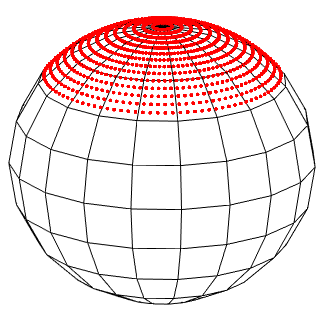
\includegraphics[width=0.306\textwidth]{figure/chapter4/k_10}}
\hfill
\subfigure[]{
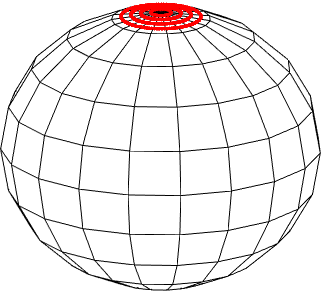
\includegraphics[width=0.306\textwidth]{figure/chapter4/k_100}}
\hfill
\subfigure[]{
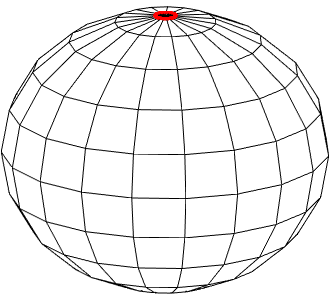
\includegraphics[width=0.306\textwidth]{figure/chapter4/k_600}}
\caption{二维球体~$\mathbb{S}^{2}$~窗函数:~(a)~$\kappa=10$,(b)~$\kappa=100$,(c)~$\kappa=600$}
\label{fig:Fishon_3D}
\end{figure}

对于~$p=2$~的一维球体~$\mathbb{S}^{1}$,Von Mises Fisher~函数的表达式为:
\begin{equation}
h(\phi)=\frac{1}{2 \pi I_{0}(\kappa)} e^{\kappa \cos \left(\phi-\phi_{0}\right)}, \quad\left|\phi-\phi_{0}\right| \leq \pi
\end{equation}
假设主瓣方向~$\phi_{0}= 0^{\circ}$,窗函数在半个空间内的分布随集中因子~$\kappa$~的变化如图~\ref{fig:Fishon_2D}~所示。综合图~\ref{fig:Fishon_3D}~和~\ref{fig:Fishon_2D}~可以看出,集中因子$\kappa$~越大,窗函数的宽度越窄,函数越集中于主瓣方向,且主瓣方向的幅值越大。
\begin{figure}[!h]
\centering
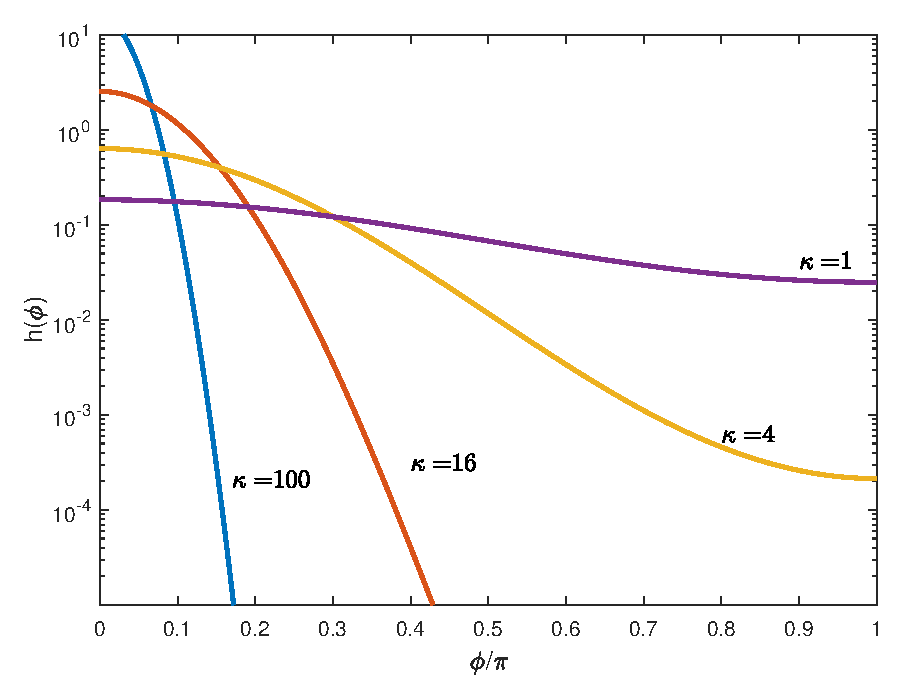
\includegraphics[width=0.6\textwidth]{figure/chapter4/FishVon_2D}
\caption{一维球体~$\mathbb{S}^{1}$~窗函数 }
\label{fig:Fishon_2D}
\end{figure}

本文中,在对原始声场进行空域加窗时,关于窗函数的选取原则如下:

(1)窗函数的主瓣方向:选取该时频点上平面波的来波方向,即球谐域~MUSIC~算法的结果;

(2)集中因子~$\kappa$:需要根据频率进行选择。设定目标半径~$R_{T}$,对于某一频率~$f$~,根据~$N_{T} = k R_{T} = 2\pi f R_{T}$~计算目标阶次,选择合适的集中因子~$\kappa$~使窗函数的球谐系数在前~$N_{T}$~阶的累积能量达到总能量的~$90\%$(或~$99\%$~等其他接近于~1~的数值)。

接下来对窗函数的球谐系数获取方法进行简单介绍。在上述选取原则的指导下,已经可以得到空域窗函数的具体表达式,因此可以在空间上任意位置取采样。相比于麦克风阵列的球谐系数获取,窗函数球谐系数的获取不受空间采样点数的限制,因此可以直接采用式~\eqref{eq.HRTF_Pinv}~的方式进行求解。


\section{整体算法框架}

基于球谐分解的双耳渲染算法直接在球谐域进行处理,如前所述,实际系统中录制声场的阶次受硬件设备的限制,因此和~HRTF~数据之间存在不匹配问题,HRTF~的直接低阶截断会对双耳信号带来损伤。本文所提出的算法分别从声场和~HRTF~两方面出发,共同解决二者之间的不匹配问题。接下来将对本文的内容进行总结,包括第~\ref{sec.SHdecomposition}~节、第~\ref{chapter.HRTF}~章和第~\ref{chapter.AddWindow}~章。


首先,第~\ref{sec.SHdecomposition}~节中对基于球谐分解的双耳渲染算法框架进行了详细介绍,给出了如何利用声场和~HRTF~的球谐系数获取双耳信号的方法。
第~\ref{chapter.HRTF}~章首先介绍了声场和~HRTF~球谐系数的获取方法,接下来引入了相位对准的~HRTF~预处理方法,并通过实验验证了该方法可以有效降低~HRTF~的球谐分解阶次。
第~\ref{chapter.AddWindow}~章创新性提出通过空域加窗的方法来提升录制声场的阶次。首先对信号模型及球谐域~MUSIC~定位算法进行了介绍,接下来对空域加窗可以实现声场阶次提升的原理进行推导,并对所采用的窗函数加以介绍。

以上三部分是本算法的理论基础,接下来给出引入声场扩阶和~HRTF~预处理的基于球谐分解的双耳渲染算法流程,如图~\ref{fig:algorithm}~所示。其中,STFT~和~ISTFT~分别为短时傅里叶变换及其逆变换,SFT~为球傅里叶变换。

\begin{figure}[H]
\centering
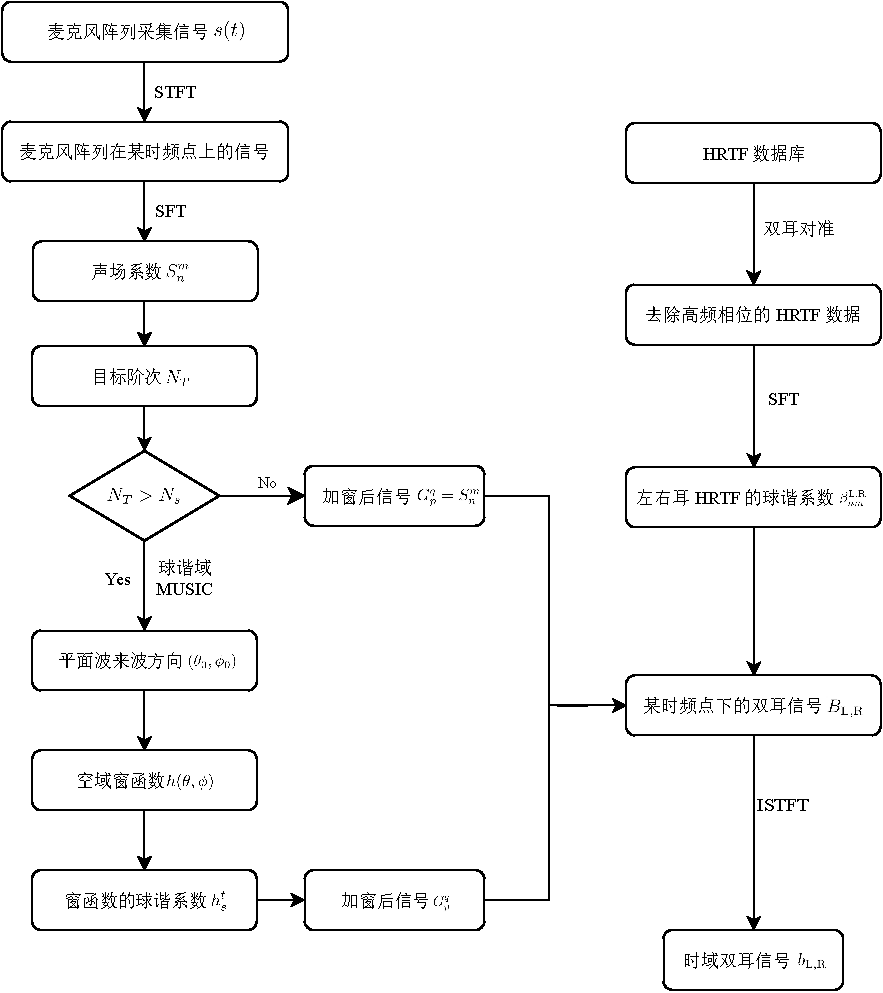
\includegraphics[width=0.88\textwidth]{figure/chapter4/algorithm}
\caption{引入声场扩阶和~HRTF~预处理的基于球谐分解的双耳渲染算法流程图}
\label{fig:algorithm}
\end{figure}

\section{本章小结}
本章对同时引入声场扩阶和~HRTF~预处理的基于球谐分解的双耳渲染算法进行了详细介绍。首先对信号模型进行描述,并给出了球谐域~MUSIC~定位算法以获取单时频点上的平面波来波方向。其次从有界线性算子出发,在球谐域上对加窗后信号的球谐系数表达式进行详细推导,并通过分析发现空域加窗可以实现声场阶次的提升。接下来对采用的窗函数及其选取原则和球谐系数求解方法加以介绍。最后将前三节的声场扩阶和第三章的~HRTF~预处理相结合,给出了总体算法框架。

